\documentclass[conference]{IEEEtran}
\IEEEoverridecommandlockouts

\usepackage{cite}
\usepackage{amsmath,amssymb,amsfonts}
\usepackage{algorithmic}
\usepackage{graphicx}
\usepackage{textcomp}
\usepackage{xcolor}
\usepackage{xcolor}
\usepackage{booktabs}
\usepackage{tabularx}
\usepackage{threeparttable}
\usepackage{xcolor}
\usepackage{multirow}
% Preamble (one-time)
\usepackage[most]{tcolorbox}
\tcbuselibrary{listings, breakable, skins}

% A full-width (double-column) prompt box with nice corners + background
\newtcblisting{FullWidthPromptBox}[2][]{%
  enhanced,
  breakable,
  float*=t,            % uses figure* to span both columns in twocolumn
  width=\textwidth,
  colback=gray!6,      % background
  colframe=black,
  colbacktitle=gray!18,
  coltitle=black,
  fonttitle=\bfseries,
  boxrule=0.9pt,
  arc=3mm,             % rounded corners
  outer arc=3mm,
  drop shadow,
  left=3mm,right=3mm,top=2mm,bottom=2mm,
  listing engine=listings,
  listing only,
  title={#2},
  listing options={
    basicstyle=\ttfamily\footnotesize,
    breaklines=true,
    breakatwhitespace=false,
    columns=fullflexible,
    keepspaces=true,
    showstringspaces=false
    % Uncomment if you want line numbers:
    % ,numbers=left, numberstyle=\tiny, stepnumber=1, numbersep=6pt
  },
  #1
}
\newcommand{\hlt}[1]{\textcolor{purple}{#1}}



\bibliographystyle{IEEEtran}


\newcommand{\ourmethod}[1]{\textcolor{black}{HALO}}
\newcommand{\rutav}[1]{\textcolor{blue}{RS: #1}}
\newcommand{\todo}[1]{\textcolor{red}{#1}}
\newcommand{\yuke}[1]{\textcolor{purple}{#1}}
\newcommand{\roberto}[1]{\textcolor{green}{#1}}

\def\BibTeX{{\rm B\kern-.05em{\sc i\kern-.025em b}\kern-.08em
    T\kern-.1667em\lower.7ex\hbox{E}\kern-.125emX}}
\begin{document}

\noindent
\textbf{Paper-ID 348.}
We thank the reviewers for recognizing our timely contribution, HALO's effectiveness, and the thoroughness of our experiments. We address the valuable feedback:

\noindent
\textbf{Comparison with MemoryVLA.} \textit{(ZkxK)}
While MemoryVLA addresses context growth via token merging, this comes at the cost of granular information retention. HALO, by contrast, stores all information and performs selective retrieval. This distinction matters: the loss of granularity can become a significant bottleneck, as shown in prior work (arXiv:2507.20198) and confirmed by our own empirical observations in two tasks, where HALO achieves \hlt{$48\%$} vs. \hlt{$20\%$} with token merging.
 
\noindent
\textbf{Additional evidence for HALO's versatility.} \textit{(ZkxK)}
We evaluate a human-robot partnership task in the real world, in which the robot observes a human perform part of the task and then completes the rest. HALO achieves \hlt{$65\%$} vs. \hlt{$20\%$} with standard attention. Together, results with four information types, two robot platforms, both simulation and real-world evaluations demonstrate HALO's versatility.
 
\noindent
\textbf{Relation of top-$k$ with context length $N$.} \textit{(ZkxK)}
\begin{figure}[h]
    \centering
    \vspace{-0.35cm}
    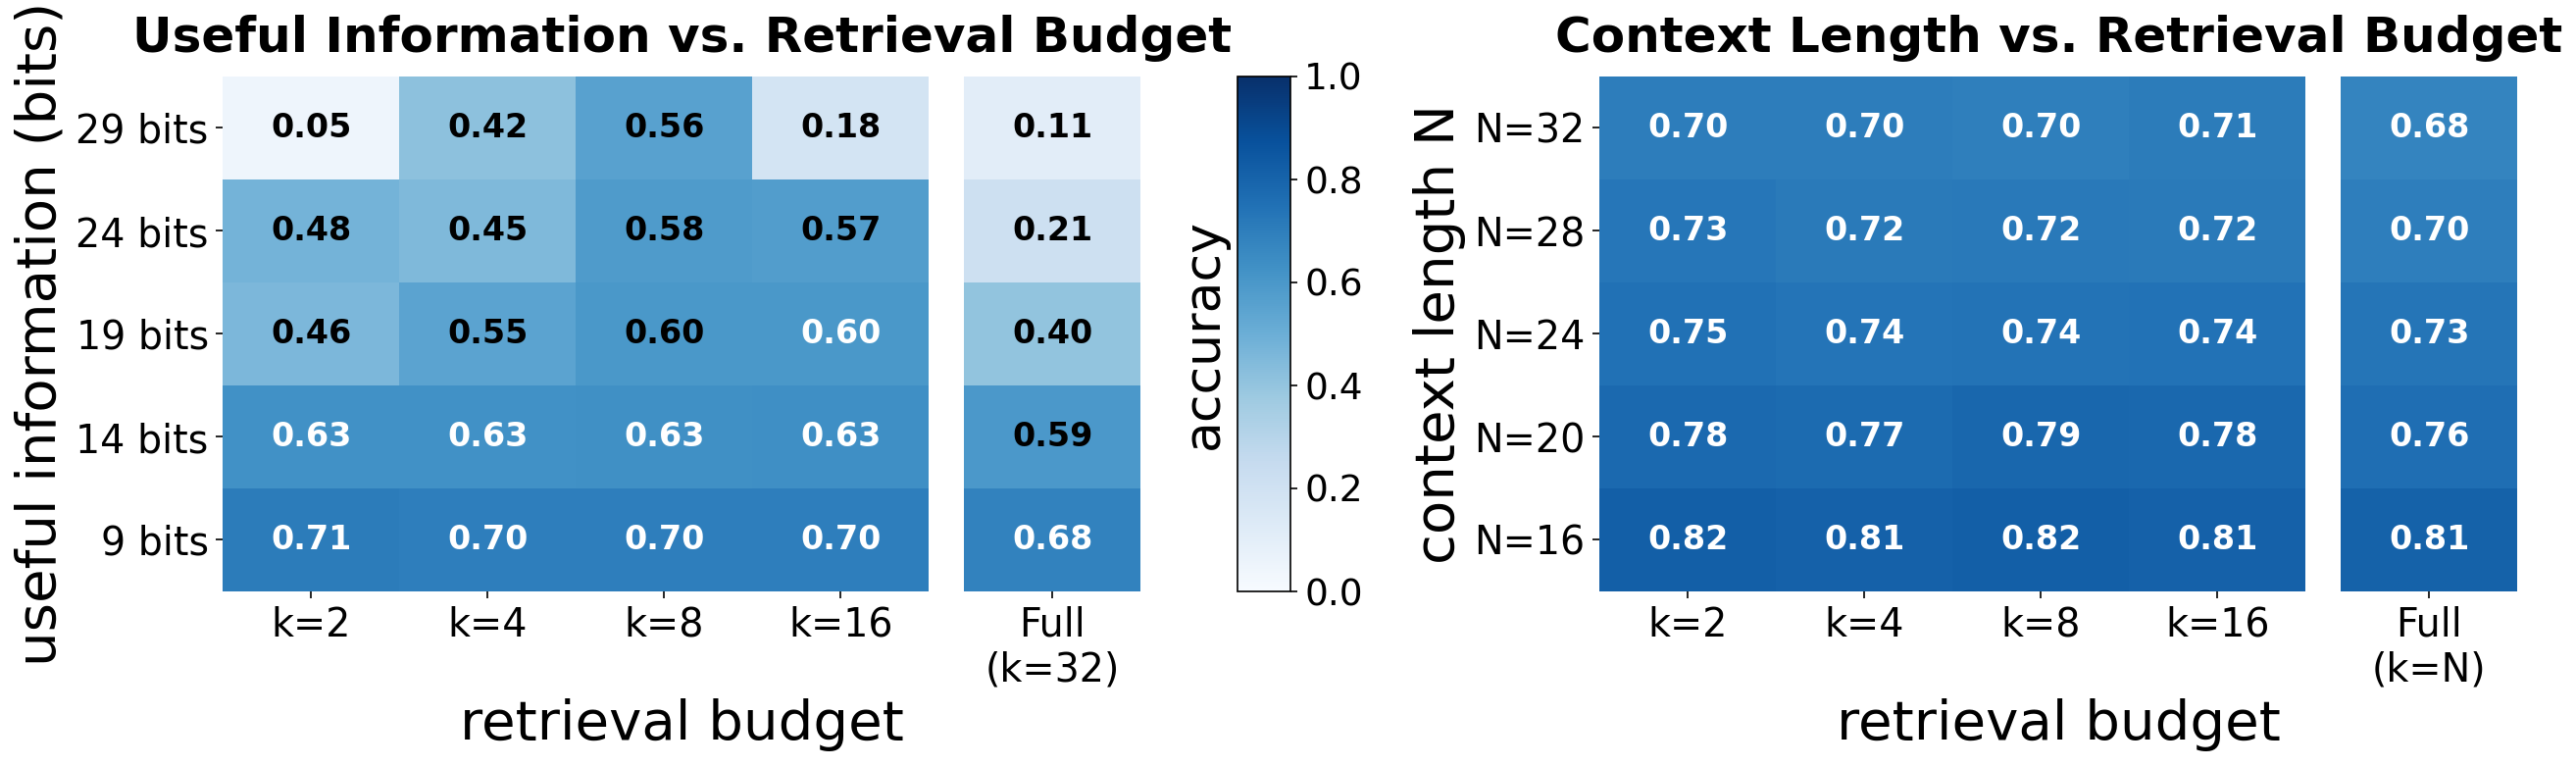
\includegraphics[width=\linewidth]{figures/k_vs_N_retrievalv2.png}
    \vspace{-0.84cm}
    \label{fig:k_ablation}
\end{figure}
The retrieval budget $k$ should depend on the information required for a decision, not the context length $N$. While isolating this in manipulation is non-trivial, we evaluate on a controlled toy dataset: for fixed $N$, performance is similar across $k$ values but varies across tasks with different information requirements.
 
\noindent
\textbf{Metric for evaluating HALO.} \textit{(gVgF, main)}
\textbf{(a)} \textit{Average performance across diverse tasks.} We acknowledge no single method wins across all tasks. However, HALO remains competitive without task-specific assumptions or hand-designed rules, making it versatile with less engineering effort across information types.
We believe average performance across tasks, alongside competitive performance on individual tasks (Tab.~1), jointly reflect this versatility.
This versatility is valuable when combining heterogeneous information for a decision; \textit{e.g.}, in `Wash and Return to Same Container,' HALO combines past visual and motion information, which hand-crafted rules miss, resulting in worse performance (App. Fig.~7).
\textbf{(b)} \textit{Additional metric of evaluation.} We measure manipulation and memory failures, finding that HALO reduces them by \hlt{$8\%$} and \hlt{$25\%$} absolute over full attention in `Retrieve Oil' task, respectively. These results support our hypothesis that HALO reduces model drift (fewer manipulation failures) and improves memory retrieval (fewer memory failures).
 
\noindent
\textbf{Comparison with text-based summaries.} \textit{(gVgF)} \textbf{P3:}
Unlike text-based memory, HALO maintains granular, multimodal memory---images, actions, and proprioceptives---preserving information that text summaries lose by design. In HALO, VQA provides priors on task-relevant information, but action prediction benefits from the full memory without being restricted to it.
The importance of granular memory is evidenced by ReMemBer (Tab.~1), which performs poorly (\hlt{$-23\%$} drop from HALO) on tasks requiring temporally granular information, such as the `Heat Pot', where the specific moment the stove was turned on is important.
 
\noindent
\textbf{VQA generation pipeline.} \textit{(gVgF)} \textbf{P11:}
% SOTA VLMs struggle to produce question--answers directly from long videos, often hallucinating objects or generating incorrect answers. To address this, HALO uses a stage-wise pipeline: (i) LLM and SAM extract per-frame granular task-relevant info., (ii) activity summarization for subtask-level info., and then (iii) combined to produce VQA pairs. Empirically, it yields $+60\%$ pts. more accurate question answers and $-20\%$ pts. fewer hallucinations compared to a single-prompt baseline.
SOTA VLMs struggle to produce question--answer pairs directly from long videos, often hallucinating objects or generating incorrect answers. To address this, HALO uses a stage-wise pipeline: (i) LLM and SAM extract per-frame granular task-relevant information, (ii) activity summarization captures subtask-level information, and (iii) both are combined to produce VQA pairs. Empirically, this yields \hlt{$+60\%$} pts. more accurate QAs and \hlt{$-20\%$} pts. fewer hallucinations compared to a single-prompt baseline.


\noindent
\textbf{Clarifications.} \textit{(gVgF)}
\textbf{P1:} In standard attention, the model may associate a decision with irrelevant context, \textit{e.g.}, the decision to retrieve oil is influenced by paper towels rather than the oil bottle (App. Fig.~8).
\textbf{P2:} Each task and its partially observable information is described in Sec.~IV.
\textbf{P4:} The top-$k$ most informative past tokens are selected via learned QKV values, shaped by gradient descent to minimize the joint objective of action prediction and VQA. Only the top-$k$ tokens, as measured by query-key similarity, influence the decision.
\textbf{P7:} We will add references for associative memory retrieval, including well-established methods using attention (arXiv:2307.15818, arXiv:2304.13705).
\textbf{P9:} \textit{E.g.}, in \textit{Wash and Return} task, full attention accumulates errors over time, leading to missed placement at the end; HALO mitigates this via top-$k$ sparsification, which suppresses the influence of accumulated errors (App. VI.D).

\noindent
\textbf{Comparison with respect top-$k$ attention and VQA in robotics.} \textit{(Rqty)}
As the reviewer highlights, HALO draws inspiration from prior work. We summarize the key distinctions. While \textbf{top-$k$ attention} is used in related domains to improve computational efficiency (arXiv:2106.06899), we are the first to apply it to mitigate model drift in long-context visuomotor policies---a non-trivial and, to our knowledge, novel application. Prior work incorporating \textbf{VQA into robot policy} training focuses on reactive policies, largely improving the model's parametric memory (arXiv:2505.23705). HALO instead uses VQA to improve both parametric and non-parametric memory; as context grows, longer non-parametric memory introduces spurious correlations, and VQA co-training helps mitigate this.
To enable this, we develop a pipeline that uses VLMs to generate memory-dependent task-relevant VQA questions.
Together, top-$k$ and VQA address challenges in long-context visuomotor policies, yielding strong performance across diverse settings.
 
\noindent
\textbf{Targeted analysis of VQA and top-$k$.} \textit{(Rqty)} We refer to App.~VI.C and VI.D for quantitative and qualitative evidence.
 
\noindent
\textbf{Addressing HALO's performance in the real world.} \textit{(Rqty)}
HALO performs poorly on two long-horizon real-world tasks (Tab.~2). We attribute this to model latency introduced by large context lengths, which creates a train-test distribution shift. Upon improving model efficiency via inference optimizations from 9~Hz to 50~Hz, we recover performance on both tasks, achieving \hlt{$55\%$} and \hlt{$70\%$}, with an avg. of \hlt{$55\%$} across all tasks.
% \textbf{Clarifications} \textit{(gVgF)}
% We provide the following clarifications in the revision:
% \begin{itemize}

% \noindent
% \textbf{Top-$k$ straight-through estimation:} \textit{(Rqty)} We apply the straight-through estimator~\cite{bengio2013estimating}, which passes gradients through all tokens in the backward pass while retaining sparse top-$k$ values in the forward pass.
% \begin{equation*}
% \texttt{x\_{topk} = x.detach() + (x\_{topk} - x\_{topk}.detach())},
% \end{equation*}
    
% \noindent
% \textbf{Model component examples:} Refer App. VI.E.
% 
% \noindent
% \textbf{References:} associative memory mechanism (e.g., attention); we note that HALO is itself an instance of associative memory; strided attention (\rutav{todo}), gated attention \rutav{todo}, 
    % \item \textbf{Training details.} \textit{(Rqty)}
%     \item \textbf{Adaptive-$k$ as future work} \textit{(ZkxK)}
% We agree that adaptive selection of $k$ is a promising direction and explicitly acknowledge it as future work in the revised manuscript.
% \end{itemize}
 
\noindent
\textit{We will incorporate all reviewers' suggestions and release the complete code for reproducibility.}


\end{document}